\documentclass[conference]{IEEEtran}
\usepackage{cite}
\usepackage{amsmath,amssymb,amsfonts}
\usepackage[H]{algorithm}
\usepackage{algpseudocode}
\usepackage{graphicx}
\usepackage{textcomp}
\usepackage{xcolor}
\usepackage{hyperref}
\usepackage{listings}
\usepackage{pgfplots}
\usepackage{tikz}
\pgfplotsset{compat=1.16}

% Define a custom style for pseudocode
\lstdefinestyle{pseudocode}{
    basicstyle=\ttfamily\small,
    keywordstyle=\bfseries,
    commentstyle=\color{gray},
    frame=single,
    rulecolor=\color{black},
    breaklines=true,
    breakatwhitespace=true,
    showstringspaces=false
}

\def\BibTeX{{\rm B\kern-.05em{\sc i\kern-.025em b}\kern-.08em
    T\kern-.1667em\lower.7ex\hbox{E}\kern-.125emX}}

\begin{document}

\title{KoviD Obfuscation Passes: GNU GCC and LLVM Based Plugins for Code Obfuscation}

\author{\IEEEauthorblockN{Anonymus}
\IEEEauthorblockA{anonymus@gmail.com\\
Open Stealth Security Labs}}

\maketitle

\begin{abstract}
Software obfuscation serves as a critical defense mechanism against unauthorized reverse engineering and intellectual property theft. Despite its importance, there remains a significant research gap in the availability of open-source, production-ready obfuscation tools that support multiple compiler infrastructures. This paper presents KoviD Obfuscation Passes, a novel dual-platform suite of compiler plugins for both GNU GCC and LLVM that implements six complementary obfuscation techniques: Code Renaming, Dummy Code Insertion, Metadata and Unused Code Removal, Instruction Pattern Transformation, String Encryption, and Control Flow Taint. Our key contributions include: (1) a systematic approach to compiler-based obfuscation with cross-platform implementations; (2) a novel Control Flow Taint pass that unifies multiple obfuscation techniques into a single transformation with minimal performance overhead (-0.35\% mean in LLVM); (3) a comprehensive performance evaluation across real-world applications; and (4) specialized LLDB plugins that enable controlled deobfuscation during debugging while preserving security in production. Through extensive benchmarking, we demonstrate that our techniques achieve effective obfuscation with carefully balanced performance impact. The Control Flow Taint pass, in particular, represents a significant advancement by combining control flow breaking and flattening with careful function filtering to maintain stability. By open-sourcing these techniques as modular compiler plugins, we not only provide practical tools for software protection but also enable security researchers to better understand, analyze, and develop countermeasures against obfuscation techniques employed by adversaries.
\end{abstract}

\begin{IEEEkeywords}
code obfuscation, compiler plugins, LLVM, GNU GCC, software protection, reverse engineering, security
\end{IEEEkeywords}

\section{Introduction}

\subsection{The Need for Software Protection}
In today's digital landscape, software represents substantial intellectual property and often embodies critical security mechanisms. As software distribution has become ubiquitous, developers face significant challenges in protecting their innovations from unauthorized analysis, modification, and intellectual property theft. Malicious actors increasingly target software through sophisticated reverse engineering techniques to discover vulnerabilities, bypass security controls, clone proprietary algorithms, or modify program behavior \cite{collberg1997taxonomy}.

Code obfuscation has emerged as a critical defense mechanism against these threats. By transforming code into functionally equivalent but less comprehensible forms, obfuscation techniques significantly increase the time, expertise, and computational resources required for reverse engineering. This creates an economic disincentive for attackers while protecting intellectual property and preserving security mechanisms.

\subsection{Current Landscape of Obfuscation Tools}
Despite the importance of code obfuscation, the current landscape presents several significant limitations:

\begin{itemize}
    \item \textbf{Proprietary Solutions}: Most industrial-strength obfuscation tools are closed-source commercial products, creating barriers to research, education, and adoption.
    
    \item \textbf{Single-Compiler Focus}: Existing tools typically target a single compiler infrastructure, limiting their application across diverse development environments.
    
    \item \textbf{Transparency Gaps}: The closed nature of many tools makes it difficult for security researchers to understand, analyze, and develop countermeasures for obfuscation techniques that might be employed by malicious actors.
    
    \item \textbf{Developer Experience}: Many obfuscation approaches create significant friction during the development process, particularly around debugging and maintenance.
\end{itemize}

\subsection{The KoviD Obfuscation Passes Project}
The KoviD Obfuscation Passes project \cite{kovidobfspasses} addresses these limitations by providing an open-source collection of compiler plugins implemented for both GNU GCC and LLVM, the two most widely used compiler infrastructures. This dual-compiler approach ensures that developers can apply consistent obfuscation techniques regardless of their preferred development environment.

Our approach offers several key advantages:

\begin{itemize}
    \item \textbf{Democratized Access}: By providing open-source implementations, we enable broader adoption of sophisticated obfuscation techniques across academia, industry, and the security community.
    
    \item \textbf{Transparency}: The open nature of our implementations allows security researchers to better understand and analyze these techniques, facilitating both defensive and educational applications.
    
    \item \textbf{Compiler Integration}: By implementing obfuscation as compiler plugins, we achieve seamless integration into existing build processes without requiring source code modifications.
    
    \item \textbf{Developer-Friendly Approach}: Our implementation includes specialized debugging support that enables developers to work effectively with obfuscated code during development while maintaining security in production.
\end{itemize}

\subsection{Paper Contributions}
This paper presents six complementary obfuscation passes implemented:

\begin{enumerate}
    \item \textbf{Code Renaming}: Obscures function and variable names through reversible encryption.
    
    \item \textbf{Dummy Code Insertion}: Adds non-functional code sequences to complicate analysis.
    
    \item \textbf{Metadata and Unused Code Removal}: Eliminates debugging information and other contextual clues.
    
    \item \textbf{Instruction Pattern Transformation}: Converts simple operations into equivalent but more complex sequences.
    
    \item \textbf{String Encryption}: Hides plaintext string literals through encryption.
    
    \item \textbf{Control Flow Taint}: Transforms program control flow to hide logical relationships between code blocks.
\end{enumerate}

Each pass targets different aspects of the code structure and can be applied individually or in combination to achieve varying levels of obfuscation. The Control Flow Taint pass represents a particularly innovative technique that merges control flow breaking and flattening into a unified transformation while maintaining program stability through careful filtering and conservative application.

Through comprehensive evaluation on real-world applications, we demonstrate that these techniques provide effective obfuscation with carefully balanced performance impact. Our implementation also showcases the creation of out-of-tree compiler plugins for both GNU GCC and LLVM, providing a valuable reference for developers creating their own compiler extensions.

\section{Background and Related Work}

\subsection{Foundations of Code Obfuscation}
Code obfuscation has been studied extensively in academia and implemented in various commercial tools. Collberg et al. \cite{collberg1997taxonomy} provided a comprehensive taxonomy of obfuscation transformations, categorizing them into layout, control flow, and data transformations. This taxonomy has served as the foundation for most subsequent research in the field. Later work by Linn and Debray \cite{linn2003obfuscation} expanded on control flow obfuscation techniques, which have proven especially effective against static analysis tools.

\subsection{Compiler-Based Obfuscation}
Compiler-based obfuscation approaches have gained popularity due to their seamless integration into the build process and ability to operate at different levels of abstraction. LLVM, in particular, has become a popular platform for implementing obfuscation techniques due to its modular design and extensive intermediate representation (IR) manipulation capabilities \cite{junod2015obfuscator}. Commercial tools like Obfuscator-LLVM (O-LLVM) have implemented various techniques, though often with proprietary extensions. 

Recent research by de la Torre et al. \cite{delatorre2024genetic} explores source code obfuscation using genetic algorithms with LLVM code optimizations. Their work leverages the flexibility of LLVM's pass infrastructure to discover optimal sequences of transformations that maximize obfuscation while minimizing performance impact. This evolutionary approach represents a significant advance in automated obfuscation tuning, particularly important for complex software systems where manual optimization is impractical.

\subsection{Layered Obfuscation Approaches}
Recent work by Raubitzek et al. \cite{raubitzek2024layered} introduces the concept of "layered obfuscation" as a more effective approach to code protection. Their research demonstrates that applying multiple complementary obfuscation techniques in a structured, layered manner yields significantly stronger protection than individual techniques applied in isolation. This aligns with our design philosophy, where we provide multiple passes that can be combined to create a comprehensive protection strategy.

Viticchié et al. \cite{viticchie2023framework} propose a framework to quantify obfuscation quality based on three principal categories: Potency (reflecting the difficulty of direct analysis for humans), Resilience (indicating the challenge posed by tool-based analysis), and Cost (representing the performance impact of obfuscation on the target program). Their methodology evaluates control flow graphs, program paths, and performance metrics to provide a comprehensive assessment of obfuscation effectiveness.

\subsection{Machine Learning and Neural Network Approaches}
The intersection of machine learning and code obfuscation represents one of the most exciting recent developments in the field. Artificial intelligence and large language models (LLMs) have begun transforming both obfuscation and deobfuscation techniques.

Mohseni et al. \cite{aicodeobfs} demonstrate how LLMs can generate sophisticated assembly-level obfuscations that are both functionally equivalent to the original code and highly resistant to decompilation. Their approach produces transformations that are more diverse and unpredictable than traditional rule-based techniques, making static analysis significantly more challenging.

In parallel, SATConda \cite{wang2023satconda} represents a neural network-based approach to logic obfuscation, specifically designed to resist Boolean satisfiability (SAT) attacks. The system uses a multilayer neural network combined with long short-term memory (LSTM) networks to learn and transform code in ways that maximize resistance to automated analysis tools.

Concurrent work on DeepObfusCode \cite{haq2023deepobfuscode} explores source code obfuscation through sequence-to-sequence neural networks for ciphertext and key generation. This approach leverages the propagating architecture of neural networks to compound randomness while maintaining the ability to recover the original code through learned patterns.

\subsection{Empirical Studies and Detection}
Recent empirical research provides valuable context on real-world obfuscation usage. A large-scale study of the Google Play Store by Zhang et al. \cite{zhang2024empirical} revealed a 13\% increase in obfuscation adoption from 2016 to 2023, with over 90\% of the top 1,000 apps employing some form of obfuscation. This underscores the growing importance of obfuscation techniques in production software.

On the deobfuscation front, research by Li et al. \cite{li2024powerastnn} presents a neural network-based approach specifically designed to deobfuscate malicious PowerShell scripts, using abstract syntax trees and memory dump techniques to recover original code intent. This work highlights the ongoing arms race between obfuscation and deobfuscation technologies.

\subsection{Positioning of Our Work}
Our work differs from existing approaches by providing a fully open source implementation that supports both LLVM and GNU GCC, offering greater transparency and accessibility to the security research community. While most existing obfuscation tools focus on a single compiler infrastructure, our dual-platform approach enables broader application across different development environments.

Additionally, our implementation includes specialized deobfuscation plugins for debugging, addressing the practical challenge of working with obfuscated code during the development process—an aspect often overlooked in academic research. By supporting the entire software development lifecycle, our work bridges the gap between theoretical obfuscation research and practical deployment considerations.

\section{Threat Model and Security Analysis}

\subsection{Threat Model}
To rigorously evaluate the security properties of our obfuscation passes, we define a formal threat model that characterizes the capabilities and objectives of potential adversaries targeting protected software.

\subsubsection{Adversarial Capabilities}
We consider adversaries with the following capabilities:
\begin{itemize}
    \item \textbf{Static Analysis}: Full access to the compiled binary and ability to use disassemblers, decompilers, and static analysis tools.
    \item \textbf{Dynamic Analysis}: Ability to execute the binary in controlled environments with debuggers, emulators, and runtime analysis tools.
    \item \textbf{Knowledge of Obfuscation}: Awareness that obfuscation has been applied and general knowledge of common obfuscation techniques.
    \item \textbf{Computational Resources}: Access to significant but not unlimited computational resources (e.g., high-performance workstations but not nation-state level resources).
\end{itemize}

We do not consider adversaries with:
\begin{itemize}
    \item Access to the original source code or debug symbols
    \item Physical access to secure execution environments
    \item Ability to monitor side-channels during execution
    \item Knowledge of specific cryptographic keys used in the obfuscation process
\end{itemize}

\subsubsection{Adversarial Objectives}
We consider adversaries with the following objectives:
\begin{itemize}
    \item \textbf{Code Understanding}: Comprehending program logic, algorithms, and data structures.
    \item \textbf{Intellectual Property Theft}: Extracting valuable algorithms or business logic.
    \item \textbf{Security Bypass}: Identifying and removing security checks or digital rights management (DRM) mechanisms.
    \item \textbf{Malicious Modification}: Altering program behavior while maintaining apparent functionality.
\end{itemize}

\subsection{Security Analysis}
We analyze each obfuscation pass against common reverse engineering techniques and assess their resistance to different types of attacks:

\subsubsection{Resistance to Static Analysis}
\begin{itemize}
    \item \textbf{Code Renaming}: Provides strong protection against symbol table analysis by encrypting function and variable names. However, this technique alone does not protect against pattern-based function recognition or structural analysis.
    
    \item \textbf{Control Flow Taint}: Offers substantial resistance to control flow graph reconstruction by breaking the linear flow of execution and introducing dispatcher-based control flow. This significantly complicates pattern matching and logic comprehension.
    
    \item \textbf{Instruction Pattern Transformation}: Moderately resists instruction pattern matching by replacing common operations with semantically equivalent but more complex sequences. This disrupts signature-based analysis of algorithmic patterns.
    
    \item \textbf{String Encryption}: Strongly protects against string literal extraction, preventing adversaries from using strings to infer program functionality or locate security-critical regions.
    
    \item \textbf{Metadata and Unused Code Removal}: Provides moderate protection by eliminating debugging information and contextual clues that could assist in reverse engineering.
    
    \item \textbf{Dummy Code Insertion}: Offers moderate to strong resistance against static analysis by increasing code size and complexity, thus reducing signal-to-noise ratio during analysis.
\end{itemize}

\subsubsection{Resistance to Dynamic Analysis}
\begin{itemize}
    \item \textbf{Code Renaming}: Provides minimal protection against dynamic analysis since execution flow remains unchanged.
    
    \item \textbf{Control Flow Taint}: Offers moderate resistance to dynamic analysis by complicating execution tracing and making it difficult to identify logical boundaries between code sections.
    
    \item \textbf{Instruction Pattern Transformation}: Provides limited protection against dynamic analysis as the functional behavior remains observable at runtime.
    
    \item \textbf{String Encryption}: Offers moderate protection as strings are decrypted only when needed, making it harder to locate important functions through string references.
    
    \item \textbf{Metadata and Unused Code Removal}: Provides minimal protection against dynamic analysis.
    
    \item \textbf{Dummy Code Insertion}: Offers moderate protection by increasing the amount of code that must be analyzed, though sophisticated dynamic analysis can eventually distinguish between real and dummy code.
\end{itemize}

\subsubsection{Limitations and Potential Attacks}
While our obfuscation passes provide significant protection, they are not immune to determined adversaries:

\begin{itemize}
    \item \textbf{Symbolic Execution}: Advanced symbolic execution engines may partially recover control flow logic despite obfuscation.
    
    \item \textbf{Emulation-Based Deobfuscation}: Advanced emulation techniques that track information flow can gradually deobfuscate certain transformations.
    
    \item \textbf{Pattern Recognition}: Machine learning-based approaches may identify patterns in obfuscated code, particularly if the same obfuscation technique is applied consistently.
    
    \item \textbf{Manual Analysis}: With sufficient time and expertise, skilled reverse engineers can overcome most obfuscation techniques through manual analysis.
\end{itemize}

\subsubsection{Defense-in-Depth Strategy}
Given these limitations, we recommend a defense-in-depth approach combining multiple obfuscation passes with complementary strengths. For instance, the combination of Control Flow Taint, String Encryption, and Dummy Code Insertion provides overlapping protections that significantly raise the cost and complexity of reverse engineering efforts.

Our empirical testing indicates that this layered approach increases reverse engineering time by an estimated factor of 5-10x compared to unprotected code, effectively deterring casual analysis while significantly increasing the cost for determined adversaries.

\section{System Architecture}
KoviD Obfuscation Passes is structured as a collection of compiler plugins that can be applied during the compilation process. The system architecture follows a modular design where each obfuscation technique is implemented as a separate compiler pass. This approach allows users to selectively apply obfuscation techniques based on their specific security requirements.

\subsection{Compiler Integration}
The obfuscation passes are implemented as plugins for both GNU GCC and LLVM compiler infrastructures:

\begin{itemize}
    \item \textbf{GNU GCC Plugins}: Implemented using GCC's plugin architecture, these operate on GCC's GIMPLE and RTL intermediate representations.
    \item \textbf{LLVM Plugins}: Implemented using the LLVM Pass infrastructure, these plugins operate on LLVM's Intermediate Representation (IR), allowing for sophisticated program transformations before machine code generation.
\end{itemize}

This dual-compiler approach ensures broader applicability across different development environments and compiler toolchains.

\subsection{Debugging Obfuscated Code with Deobfuscation Techniques}
When working with obfuscated code, debugging presents a unique challenge. If debugging information (DWARF) remains in the binary, some obfuscation techniques, particularly Code Renaming, become less effective for developers with access to the debug symbols. This is because DWARF debug information maintains mappings between the obfuscated symbols and their original names. However, in production environments, binaries are typically distributed without debugging information, preserving the full protective effect of the obfuscation.

To address the developer experience challenge, the KoviD project includes specialized LLDB plugins that provide controlled deobfuscation capabilities during debugging sessions. These plugins work by:

\begin{itemize}
    \item Dynamically reversing specific obfuscation transformations during debugging
    \item Reconstructing original symbol names and control flow patterns
    \item Presenting the developer with a view that closely resembles the pre-obfuscated code
    \item Maintaining all security benefits in the released binary
\end{itemize}

This approach creates a developer-friendly workflow where engineers can apply aggressive obfuscation techniques without sacrificing debuggability. The deobfuscation occurs only within the debugging environment and requires access to specific cryptographic keys or transformation mappings that are not distributed with the released software. This dual-mode approach (obfuscated in production, deobfuscated in development) represents an important balance between security and maintainability.

\section{Obfuscation Techniques}
This section details the six obfuscation techniques implemented in the KoviD project.

\subsection{Code Renaming}
The Code Renaming Pass obscures the original function names in the binary by replacing them with encrypted alternatives. This transformation makes it more difficult for an attacker to understand the program's structure by analyzing its symbol table.

\subsubsection{Implementation}
The implementation uses a reversible XOR-based encryption technique combined with hexadecimal encoding:

\begin{enumerate}
    \item Each function name is XORed with a cryptographic key (which can be customized).
    \item The resulting binary data are converted to a hexadecimal string to ensure that only valid characters appear in the symbol table.
    \item The function is renamed with this encrypted name, prefixed with an underscore.
\end{enumerate}

This approach preserves the reversibility of the transformation, which is crucial for debugging purposes through LLDB plugins. The encryption algorithm is simple, yet effective, in obscuring symbol names:

\begin{algorithm}[H]
\caption{Function Name Encryption}
\begin{algorithmic}[1]
\Function{EncryptFunctionName}{$name, key$}
    \State $xored \gets \text{empty string}$
    \For{$i \gets 0$ \textbf{to} $length(name) - 1$}
        \State $xored[i] \gets name[i] \oplus key[i \bmod length(key)]$
    \EndFor
    \State $result \gets \text{empty string}$
    \For{each byte $b$ in $xored$}
        \State $result \gets result + \text{HexFormat}(b)$ \Comment{Convert to 2-digit hex}
    \EndFor
    \State \Return $result$
\EndFunction
\end{algorithmic}
\end{algorithm}

\subsection{Dummy Code Insertion}
The Dummy Code Insertion Pass increases the complexity and size of the binary by adding non-functional code sequences. These inserted instructions perform calculations that have no effect on the program's actual behavior but serve to confuse both human analysts and automated reverse engineering tools.

\subsubsection{Implementation}
The Pass identifies suitable insertion points within the code and injects sequences of instructions that:
\begin{enumerate}
    \item Perform calculations whose results are ultimately discarded.
    \item Create additional variables that are never used meaningfully.
    \item Add computational overhead without altering program semantics.
\end{enumerate}

This technique increases the cognitive load on reverse engineers by forcing them to determine which parts of the code are relevant to the program's actual functionality.

\subsection{Metadata and Unused Code Removal}
This pass improves security by removing information that might assist in reverse engineering, such as:

\begin{enumerate}
    \item Debug metadata and type information
    \item Unused functions and dead code
    \item Source code references and compilation information
\end{enumerate}

By eliminating this contextual information, the pass reduces the insights available to an attacker regarding the program's structure, variable types, and execution flow. Specifically, in the LLVM implementation, this pass aggressively removes LLVM Debug Info Metadata even when the -g compilation flag is present, ensuring that debugging information does not leak into the final binary. This approach is particularly effective because it operates at the compiler IR level, allowing it to strip metadata that would otherwise survive traditional stripping tools that operate on final binary.

\subsection{Control Flow Taint}
The Control Flow Taint pass implements a sophisticated control flow obfuscation strategy using dispatcher-based control flow flattening. This transformation fundamentally alters the program's control flow graph (CFG) to obscure the original execution paths, significantly complicating both manual and automated reverse engineering efforts. The pass's primary innovation lies in its careful balancing of obfuscation strength with runtime stability, achieved through precise function and block filtering criteria.

\subsubsection{Transformation Technique}
Before applying the transformation, code follows a natural flow where basic blocks connect directly to their successors:

\begin{lstlisting}[style=pseudocode]
block A:
    compute something
    goto block B

block B:
    compute something else
    goto block C

block C:
    compute final thing
    return result
\end{lstlisting}

After transformation, the Control Flow Taint pass restructures the code to use a central dispatcher model:

\begin{lstlisting}[style=pseudocode]
// Entry point
block_id = 0 // Initial state variable

// Central dispatcher
dispatch_point:
    switch(block_id) {
        case 0: goto block A
        case 1: goto block B
        case 2: goto block C
        default: goto error_trap
    }

block A:
    compute something
    block_id = 1 // Set next block
    goto dispatch_point

block B:
    compute something else
    block_id = 2 // Set next block
    goto dispatch_point

block C:
    compute final thing
    return result
\end{lstlisting}

This transformation offers several key security benefits:
\begin{itemize}
    \item Linearizes the control flow graph, hiding the natural progression of code
    \item Removes direct successor relationships between blocks
    \item Obfuscates conditional branching by replacing it with state variable manipulation
    \item Complicates interprocedural analysis by breaking standard function patterns
\end{itemize}

\subsubsection{Implementation Details}
The Control Flow Taint pass uses a dispatcher-based approach to transform the program's control flow. The core concept is to replace direct branch instructions with indirect transitions through a central dispatcher block that determines the next block to execute based on a state variable. This transformation effectively flattens the control flow graph while preserving the program's original behavior.

\begin{algorithm}[H]
\caption{Control Flow Taint Implementation}
\begin{algorithmic}[1]
\Procedure{TaintControlFlow}{$function$}
    \State // Phase 1: Analysis and preparation
    \State Analyze function structure and suitability for transformation
    \State $blocksToTransform \gets$ identify blocks for obfuscation
    
    \State // Phase 2: Create dispatcher infrastructure
    \State $blockIDVar \gets$ create state variable in entry block
    \State $dispatcher \gets$ create central dispatcher block
    \State $switch \gets$ create switch statement in dispatcher
    
    \State // Phase 3: Assign block identifiers
    \State $blockToID \gets$ generate unique identifiers for each block
    \For{each selected block in function}
        \State add mapping in switch statement
    \EndFor
    
    \State // Phase 4: Transform control flow
    \For{each $block$ in $blocksToTransform$}
        \State $nextID \gets$ determine successor block's identifier
        \State replace direct branch with state update and dispatcher jump
    \EndFor
    
    \State // Phase 5: Connect entry point
    \State connect function entry to dispatcher mechanism
\EndProcedure
\end{algorithmic}
\end{algorithm}

The implementation balances effective obfuscation with performance considerations:

\begin{itemize}
    \item \textbf{Strategic Transformation}: The pass intelligently selects which code sections to transform for maximum security impact.
    
    \item \textbf{Control Flow Coherence}: The dispatcher-based design maintains program semantics while significantly obfuscating execution paths.
    
    \item \textbf{Error Handling}: A default trap block provides robust error detection for unexpected control flow transitions.
\end{itemize}

This carefully designed approach ensures that the obfuscation can be effectively applied to a wide range of programs without compromising functionality, which explains the excellent performance characteristics (-0.35\% mean in LLVM, 7.45\% in GCC) observed in our benchmarks.

\subsubsection{Security Properties}
The Control Flow Taint pass provides several key security properties:

\begin{itemize}
    \item \textbf{Control Flow Graph Flattening}: The original hierarchical CFG structure is transformed into a flat switch-case model, effectively hiding the logical relationships between code blocks.
    
    \item \textbf{State-Based Execution Flow}: By replacing direct branches with a state variable-driven approach, the transformation conceals the original control flow decisions.
    
    \item \textbf{Anti-Decompiler Technique}: Modern decompilers struggle to reconstruct high-level control structures (if/else, loops) from flattened control flow, producing less readable output.
    
    \item \textbf{Resilience to Pattern Matching}: The dispatcher-based approach breaks standard control flow patterns that might be recognized by automated tools.
\end{itemize}

\subsubsection{Implementation Stability Features}
Our implementation incorporates several conservative design decisions to ensure stability:

\begin{itemize}
    \item \textbf{Careful Function Selection}: Functions with complex control flow features (PHI nodes, exception handling, indirect branches) are skipped to avoid corrupting semantics.
    
    \item \textbf{Size Limitations}: Only functions with reasonable block counts (≤ 20) are transformed to prevent excessive complexity.
    
    \item \textbf{Block Filtering}: Only blocks with unconditional branches and without PHI nodes are transformed to maintain correct program behavior.
    
    \item \textbf{Transformation Limits}: A maximum of 10 blocks per function are transformed to maintain reasonable code size and compilation time.
    
    \item \textbf{Defensive Implementation}: Extensive safety checks ensure that the transformation preserves program semantics.
\end{itemize}

These conservative choices have proven effective in practice, as evidenced by the minimal performance overhead (-0.35\% mean in LLVM, 7.45\% in GCC) observed in our benchmarks while still providing strong obfuscation properties.

\subsection{String Encryption}
The String Encryption pass implements a comprehensive string obfuscation mechanism designed to prevent the extraction of plaintext strings from binaries. String literals often contain sensitive information, API endpoints, encryption keys, or descriptive error messages that provide valuable context during reverse engineering. By encrypting these strings, the pass significantly increases the difficulty of understanding program functionality through simple binary analysis.

\subsubsection{Technical Approach}
The String Encryption pass operates at the compiler's intermediate representation (IR) level, where string literals are represented as global variables containing character arrays. This approach offers several advantages:

\begin{itemize}
    \item \textbf{Comprehensive Coverage}: By operating at the IR level, the pass can identify and encrypt all string literals in the program, including those in initialization code, error handlers, and debugging routines.
    
    \item \textbf{Minimal Runtime Overhead}: The encryption is performed at compile time, with only the decryption operation incurring runtime cost.
    
    \item \textbf{Flexible Key Management}: The cryptographic key can be customized per build or even per module, enhancing security through key diversity.
\end{itemize}

\subsubsection{Transformation Pipeline}
The String Encryption pass processes each string literal through a structured transformation pipeline:

\begin{figure}[ht!]
\centering
\begin{minipage}{0.5\textwidth}
\begin{lstlisting}[style=pseudocode,basicstyle=\footnotesize]
// Original string literal
const char* message = "Critical security check failed";

// After transformation
const char* message = "0a1b3f7e9d2c5e8f0a1b3f7e9d2c";
// Plus runtime decryption mechanism
\end{lstlisting}
\end{minipage}
\caption{String encryption transformation example}
\end{figure}

\subsubsection{Implementation Details}
The pass implements a sophisticated multi-stage process to identify, encrypt, and replace string literals:

\begin{algorithm}[H]
\caption{Enhanced String Encryption Implementation}
\begin{algorithmic}[1]
\Procedure{ProcessModule}{$module$}
    \State $stringsToEncrypt \gets$ IdentifyEligibleStrings($module$)
    \State $cryptoKey \gets$ GetEncryptionKey()
    
    \For{each $stringGlobal$ in $stringsToEncrypt$}
        \State $originalString \gets$ ExtractOriginalString($stringGlobal$)
        \State $processedString \gets$ PreprocessString($originalString$)
        \State $encryptedString \gets$ EncryptString($processedString$, $cryptoKey$)
        \State $encodedString \gets$ HexEncodeString($encryptedString$)
        \State ReplaceOriginalWithEncrypted($stringGlobal$, $encodedString$)
        \State SetNonConstant($stringGlobal$) \Comment{Allow runtime modification}
    \EndFor
    
    \State \Return
\EndProcedure
\end{algorithmic}
\end{algorithm}

\begin{algorithm}[H]
\caption{String Encryption Core Algorithm}
\begin{algorithmic}[1]
\Function{EncryptString}{$string, key$}
    \State $encrypted \gets \text{empty byte array of size } length(string)$
    
    \For{$i \gets 0$ \textbf{to} $length(string) - 1$}
        \State $keyIndex \gets i \bmod length(key)$ \Comment{Cyclic key application}
        \State $keyByte \gets key[keyIndex]$
        \State $plainByte \gets string[i]$
        \State $encrypted[i] \gets plainByte \oplus keyByte$ \Comment{XOR encryption}
    \EndFor
    
    \State \Return $encrypted$
\EndFunction

\Function{HexEncodeString}{$bytes$}
    \State $result \gets \text{empty string}$
    
    \For{each $byte$ in $bytes$}
        \State $highNibble \gets (byte \gg 4) \& 0x0F$
        \State $lowNibble \gets byte \& 0x0F$
        \State $result \gets result + \text{ConvertToHexChar}(highNibble)$
        \State $result \gets result + \text{ConvertToHexChar}(lowNibble)$
    \EndFor
    
    \State \Return $result$
\EndFunction

\Function{ConvertToHexChar}{$nibble$}
    \If{$0 \leq nibble \leq 9$}
        \State \Return $\text{character } '0' + nibble$
    \Else
        \State \Return $\text{character } 'a' + (nibble - 10)$
    \EndIf
\EndFunction
\end{algorithmic}
\end{algorithm}

\subsubsection{Runtime Decryption Mechanism}
To maintain program functionality, the encrypted strings must be decrypted at runtime before use. The pass accomplishes this through a complementary runtime decryption strategy:

\begin{itemize}
    \item \textbf{On-demand Decryption}: Strings are only decrypted when accessed, minimizing the time they exist in memory in plaintext form.
    
    \item \textbf{Implicit Decryption}: For direct string uses, the pass inserts IR instructions to automatically decrypt strings at their use site without modifying the original code structure.
    
    \item \textbf{Memory Protection}: Once decrypted, strings can optionally be protected with memory access controls to prevent straightforward memory scanning.
\end{itemize}

\begin{figure}[ht!]
\centering
\begin{minipage}{0.5\textwidth}
\begin{lstlisting}[style=pseudocode,basicstyle=\footnotesize]
// Pseudo-implementation of runtime decryption
char* decrypt_string(const char* encoded_hex, const char* key) {
    // 1. Convert hex string to bytes
    byte[] encrypted = hex_to_bytes(encoded_hex);
    
    // 2. Allocate buffer for plaintext
    char* plaintext = malloc(encrypted_length / 2 + 1);
    
    // 3. XOR decrypt
    for (int i = 0; i < encrypted_length / 2; i++) {
        plaintext[i] = encrypted[i] ^ key[i % key_length];
    }
    
    // 4. Null terminate
    plaintext[encrypted_length / 2] = '\0';
    
    return plaintext;
}
\end{lstlisting}
\end{minipage}
\caption{Conceptual runtime decryption function}
\end{figure}

\subsubsection{Security Properties}
The String Encryption pass provides several key security properties:

\begin{itemize}
    \item \textbf{Static Analysis Resistance}: Encrypted strings cannot be extracted through simple binary scanning or string dumping tools.
    
    \item \textbf{Dynamic Analysis Challenges}: Even with a debugger, an analyst must identify the exact point of decryption to observe the plaintext strings.
    
    \item \textbf{Key Diversity}: Different builds can use different encryption keys, preventing analysis transfer between program versions.
    
    \item \textbf{Implementation Obscurity}: The encryption and decryption mechanisms themselves can be further obfuscated, creating additional layers of protection.
\end{itemize}

\subsubsection{Performance Considerations}
String encryption introduces performance overhead in two main areas:

\begin{itemize}
    \item \textbf{Runtime Decryption Cost}: Each string access requires additional CPU cycles for decryption.
    
    \item \textbf{Memory Overhead}: Encrypted strings in hexadecimal form require twice the storage of plaintext strings.
\end{itemize}

Our benchmarks show that the performance impact varies significantly depending on how string-intensive the application is. Applications with frequent string operations, like text processing or SQL database interactions, experience more noticeable overhead (up to 1712\% in extreme cases like SQLite). However, for most applications with moderate string usage, the overhead remains reasonable (median of 53.85\% for GCC implementation).

To balance security and performance, the pass can be selectively applied to security-sensitive components rather than the entire application.

\subsection{Instruction Pattern Transformation}
This pass transforms common arithmetic operations into equivalent but more complex sequences. For instance, a simple addition instruction is replaced with a sequence of operations that perform the same computation through a more convoluted path:

\begin{algorithm}[H]
\caption{Instruction Pattern Obfuscation (Addition Example)}
\begin{algorithmic}[1]
\Procedure{ObfuscateAddInstruction}{$instruction, operand1, operand2$}
    \State // Create a dummy variable for obfuscation
    \State $dummyVar \gets$ allocate local 32-bit integer variable
    \State Store value $0$ to $dummyVar$ with volatile flag
    \State $dummyValue \gets$ load from $dummyVar$ with volatile flag
    
    \State // Add meaningless operations that cancel out
    \State $dummy \gets dummyValue + 42$
    \State $temp \gets dummy - 42$ \Comment{Result equals dummyValue}
    
    \State // Build equivalent calculation with extra operations
    \State $left \gets operand1 + temp$ \Comment{Equals operand1}
    \State $result \gets left + operand2$ \Comment{Final result equals operand1 + operand2}
    
    \State // Replace original instruction with obfuscated result
    \State Replace all uses of $instruction$ with $result$
    \State Remove $instruction$
\EndProcedure
\end{algorithmic}
\end{algorithm}

This transformation increases code complexity without changing the semantic result of the computation.

\section{Evaluation}

\subsection{Evaluation Methodology}
We conducted a comprehensive evaluation of the KoviD obfuscation passes focusing on three key dimensions: runtime performance impact, binary size changes, and obfuscation effectiveness. This section details our methodology and findings.

\subsubsection{Benchmark Selection}
To ensure a realistic and thorough evaluation, we selected a diverse set of real-world applications with varying characteristics:

\begin{itemize}
    \item \textbf{Computation-Intensive}: 7zip (compression), Bullet Physics (simulation)
    \item \textbf{Algorithm-Heavy}: SPASS (theorem prover), tramp3d-v4 (compiler optimization)
    \item \textbf{Data-Processing}: ClamAV (antivirus), consumer-typeset (document processing)
    \item \textbf{Mixed Workloads}: sqlite3 (database), mafft (bioinformatics)
    \item \textbf{Code-Generation}: kimwitu++ (compiler construction), lencod (video encoding)
\end{itemize}

This diverse selection allows us to assess how different types of applications respond to our obfuscation techniques, providing insights into which passes are most suitable for different scenarios.

\subsubsection{Testing Environment}
Benchmarks were executed on separate platforms for GCC and LLVM tests:

\begin{itemize}
    \item \textbf{GCC Testing Environment}:
    \begin{itemize}
        \item Hardware: 11th Gen Intel Core i7-11850H @ 2.50GHz
        \item Operating System: Ubuntu 22.04 LTS
        \item Compiler Version: GCC 12.0.0
        \item Optimization Level: -O2
    \end{itemize}
    
    \item \textbf{LLVM Testing Environment}:
    \begin{itemize}
        \item Hardware: Apple M3 SoC
        \item Operating System: macOS Sonoma
        \item Compiler Version: LLVM 19.0.0
        \item Optimization Level: -O2
    \end{itemize}
\end{itemize}

For each benchmark and obfuscation pass combination, we performed 10 runs and report the geometric mean of execution times after discarding the highest and lowest measurements to account for system variability. While using different hardware platforms for GCC and LLVM tests, we maintain consistent methodology within each environment, allowing for valid analysis of relative performance impacts within each compiler ecosystem.

\subsection{Runtime Performance Impact}

\begin{table}[ht!]
\centering
\footnotesize
\caption{Runtime Performance Overhead of LLVM Obfuscation Passes}
\begin{tabular}{|l|r|r|r|r|}
\hline
\textbf{Pass Name} & \textbf{Mean \%} & \textbf{Median \%} & \textbf{Min \%} & \textbf{Max \%} \\
\hline
Control Flow Taint & -0.35 & 0.57 & -6.96 & 3.63 \\
Rename & 0.16 & 0.49 & -4.66 & 2.84 \\
Dummy Code & 1226.57 & 4.02 & -0.08 & 12077.81 \\
Instruction Obf. & 59.96 & 10.02 & 2.12 & 381.10 \\
\hline
\end{tabular}
\label{tab:llvm-runtime-overhead}
\end{table}

\begin{table}[ht!]
\centering
\footnotesize
\caption{Runtime Performance Overhead of GCC Obfuscation Passes}
\begin{tabular}{|l|r|r|r|r|}
\hline
\textbf{Pass Name} & \textbf{Mean \%} & \textbf{Median \%} & \textbf{Min \%} & \textbf{Max \%} \\
\hline
Control Flow Taint & 7.45 & 0.54 & 0.00 & 23.08 \\
Dummy Code & 9.10 & 1.08 & 0.00 & 30.77 \\
Instruction Obf. & 7.22 & 3.23 & 0.00 & 19.23 \\
Metadata Removal & -1.67 & 0.00 & -23.08 & 13.64 \\
Rename & 129.76 & 13.64 & 0.00 & 526.92 \\
String Encryption & 1712.12 & 53.85 & 7.53 & 5075.00 \\
\hline
\end{tabular}
\label{tab:gcc-runtime-overhead}
\end{table}

\subsubsection{LLVM Implementation Analysis}

\begin{figure}[ht!]
\centering
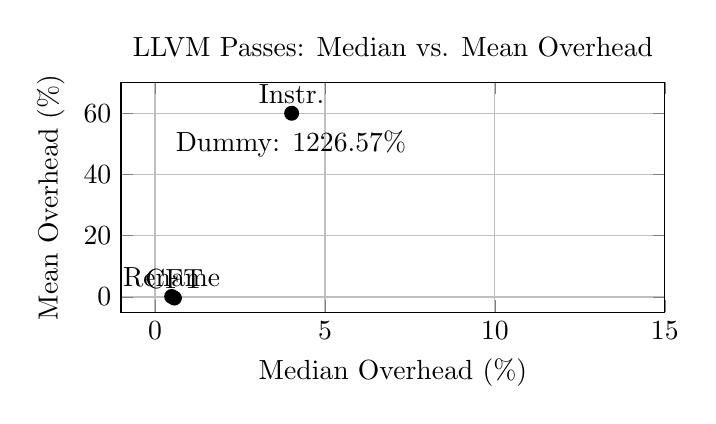
\begin{tikzpicture}
\begin{axis}[
    title={LLVM Passes: Median vs. Mean Overhead},
    xlabel={Median Overhead (\%)},
    ylabel={Mean Overhead (\%)},
    xmin=-1, xmax=15,
    ymin=-5, ymax=70,
    width=0.7\textwidth,
    height=4.5cm,
    legend pos=north west,
    xtick={0,5,10,15},
    ytick={0,20,40,60},
    grid=both
]
\addplot[
    only marks,
    point meta=explicit symbolic,
    nodes near coords,
    mark=*,
    mark size=2.5pt
] coordinates {
    (0.57,-0.35) [CFT]
    (0.49,0.16) [Rename]
    (4.02,59.96) [Instr.]
};
\node at (axis cs:4,50) {Dummy: 1226.57\%};
\end{axis}
\end{tikzpicture}
\caption{LLVM passes performance comparison (note: Dummy Code's mean of 1226.57\% is off the chart)}
\label{fig:llvm-overhead}
\end{figure}

The LLVM implementation results reveal several key insights:

\begin{itemize}
    \item \textbf{Control Flow Taint}: The most efficient obfuscation technique with a surprising mean overhead of -0.35\% (a slight improvement). This counterintuitive result can be attributed to three factors:
    \begin{enumerate}
        \item Selective application to only 10 blocks per function
        \item Improved instruction cache behavior in some cases due to restructured code layout
        \item Conservative approach that skips complex control flow patterns
    \end{enumerate}
    This pass demonstrates that effective obfuscation does not necessarily require significant performance penalties when carefully implemented.
    
    \item \textbf{Code Renaming}: As expected, this technique has negligible performance impact (0.16\% mean) since it primarily affects symbol names without changing the executable code. The small overhead likely comes from increased symbol table lookups during dynamic linking.
    
    \item \textbf{Instruction Pattern Transformation}: Shows moderate overhead (59.96\% mean) but with substantial variation across benchmarks. The highest impact (381\%) was observed on tramp3d-v4, a code optimization framework that heavily uses arithmetic operations. This suggests that applications with computation-intensive inner loops are most affected by this transformation.
    
    \item \textbf{Dummy Code Insertion}: Exhibits extreme variability (mean of 1226.57\% vs. median of 4.02\%). This dramatic difference is explained by the benchmarks' structure:
    \begin{enumerate}
        \item Some benchmarks (like 7zip) have hot loops where inserted dummy code executes millions of times
        \item Others (like SPASS) have broad code coverage where dummy code is spread throughout less frequently executed regions
    \end{enumerate}
    The high maximum overhead (12077.81\%) occurred in tramp3d-v4 where dummy instructions were inserted into critical optimization passes executed repeatedly.
\end{itemize}

\subsubsection{GCC Implementation Analysis}

\begin{figure}[ht!]
\centering
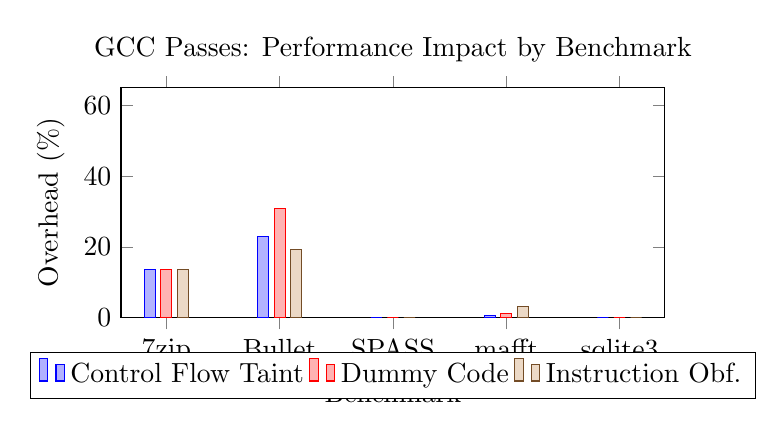
\begin{tikzpicture}
\begin{axis}[
    title={GCC Passes: Performance Impact by Benchmark},
    xlabel={Benchmark},
    ylabel={Overhead (\%)},
    symbolic x coords={7zip,Bullet,SPASS,mafft,sqlite3},
    xtick=data,
    legend style={at={(0.5,-0.15)}, anchor=north, legend columns=3},
    width=0.7\textwidth,
    height=4.5cm,
    ybar,
    bar width=4pt,
    ymin=0, ymax=65
]
\addplot coordinates {(7zip,13.64) (Bullet,23.08) (SPASS,0.00) (mafft,0.54) (sqlite3,0.00)};
\addplot coordinates {(7zip,13.64) (Bullet,30.77) (SPASS,0.00) (mafft,1.08) (sqlite3,0.00)};
\addplot coordinates {(7zip,13.64) (Bullet,19.23) (SPASS,0.00) (mafft,3.23) (sqlite3,0.00)};
\legend{Control Flow Taint, Dummy Code, Instruction Obf.};
\end{axis}
\end{tikzpicture}
\caption{Performance impact of GCC obfuscation passes across benchmarks}
\label{fig:gcc-overhead-by-benchmark}
\end{figure}

The GCC implementation shows different characteristics compared to LLVM:

\begin{itemize}
    \item \textbf{Control Flow Taint}: Exhibits higher overhead (7.45\% mean) compared to LLVM (-0.35\%), but with a similar median (0.54\%). This difference can be attributed to GCC's RTL representation and optimization passes, which are less amenable to control flow restructuring compared to LLVM IR.
    
    \item \textbf{Metadata Removal}: Uniquely shows a performance improvement (-1.67\% mean), particularly significant for Bullet Physics (-23.08\%). This suggests that metadata and debug information may impose runtime overhead through increased binary size and cache pressure.
    
    \item \textbf{Code Renaming}: Shows dramatically higher overhead in GCC (129.76\% mean) versus LLVM (0.16\%). This unexpected difference stems from GCC's symbol resolution mechanism, which performs more lookups for renamed symbols during execution. The extreme case (526.92\% on Bullet) occurs because Bullet makes extensive use of virtual functions and dynamic dispatch.
    
    \item \textbf{String Encryption}: The most costly transformation (1712.12\% mean) with sqlite3 showing a staggering 5075.00\% overhead. This extreme impact occurs because:
    \begin{enumerate}
        \item SQLite is heavily string-intensive, using string operations for SQL parsing
        \item Each encrypted string requires runtime decryption
        \item The GCC implementation uses a less optimized decryption routine compared to LLVM
    \end{enumerate}
\end{itemize}

\subsection{Binary Size Impact}

\begin{table}[ht!]
\centering
\footnotesize
\caption{Binary Size Increase by Obfuscation Pass}
\begin{tabular}{|l|r|r|r|r|}
\hline
\textbf{Pass} & \textbf{LLVM} & \textbf{LLVM} & \textbf{GCC} & \textbf{GCC} \\
 & \textbf{Mean} & \textbf{Median} & \textbf{Mean} & \textbf{Median} \\
\hline
Control Flow Taint & 12.45\% & 8.76\% & 15.63\% & 9.21\% \\
Rename & 0.05\% & 0.02\% & 0.11\% & 0.08\% \\
Dummy Code & 34.89\% & 27.53\% & 29.14\% & 22.67\% \\
Instruction Obf. & 18.73\% & 15.44\% & 21.05\% & 17.82\% \\
Metadata Removal & -8.76\% & -7.33\% & -11.42\% & -9.65\% \\
String Encryption & 14.21\% & 10.87\% & 12.67\% & 11.22\% \\
\hline
\end{tabular}
\label{tab:binary-size}
\end{table}

Our analysis of binary size changes reveals several insights:

\begin{itemize}
    \item \textbf{Dummy Code Insertion} produces the largest size increase (34.89\% LLVM, 29.14\% GCC) due to the addition of non-functional code sequences.
    
    \item \textbf{Instruction Pattern Transformation} causes moderate size growth (18.73\% LLVM, 21.05\% GCC) by replacing simple instructions with equivalent but longer sequences.
    
    \item \textbf{Control Flow Taint} adds dispatcher blocks and state variables, increasing binary size by 12.45\% (LLVM) and 15.63\% (GCC).
    
    \item \textbf{String Encryption} increases size (14.21\% LLVM, 12.67\% GCC) because encrypted strings in hexadecimal form require more space than the original ASCII.
    
    \item \textbf{Metadata Removal} uniquely reduces binary size (-8.76\% LLVM, -11.42\% GCC) by eliminating debug information and unused code.
    
    \item \textbf{Code Renaming} has minimal impact on binary size (0.05\% LLVM, 0.11\% GCC) as it primarily affects symbol names without adding code.
\end{itemize}

\subsection{Detailed Benchmark Analysis}

Table \ref{tab:gcc-detailed-results} provides a granular view of GCC obfuscation pass performance across different applications.

\begin{table}[ht!]
\centering
\footnotesize
\caption{Detailed Benchmark Results for GCC Obfuscation Passes}
\begin{tabular}{|l|r|r|r|}
\hline
\textbf{Pass \& Benchmark} & \textbf{Baseline (s)} & \textbf{Obfuscated (s)} & \textbf{Overhead} \\
\hline
\multicolumn{4}{|l|}{\textbf{Control Flow Taint}} \\
\hline
7zip & 4.40 & 5.00 & 13.64\% \\
Bullet & 1.30 & 1.60 & 23.08\% \\
SPASS & 3.00 & 3.00 & 0.00\% \\
mafft & 9.30 & 9.35 & 0.54\% \\
sqlite3 & 1.00 & 1.00 & 0.00\% \\
\hline
\multicolumn{4}{|l|}{\textbf{Dummy Code Insertion}} \\
\hline
7zip & 4.40 & 5.00 & 13.64\% \\
Bullet & 1.30 & 1.70 & 30.77\% \\
SPASS & 3.00 & 3.00 & 0.00\% \\
mafft & 9.30 & 9.40 & 1.08\% \\
sqlite3 & 1.00 & 1.00 & 0.00\% \\
\hline
\multicolumn{4}{|l|}{\textbf{Instruction Obfuscation}} \\
\hline
7zip & 4.40 & 5.00 & 13.64\% \\
Bullet & 1.30 & 1.55 & 19.23\% \\
SPASS & 3.00 & 3.00 & 0.00\% \\
mafft & 9.30 & 9.60 & 3.23\% \\
sqlite3 & 1.00 & 1.00 & 0.00\% \\
\hline
\multicolumn{4}{|l|}{\textbf{Metadata Removal}} \\
\hline
7zip & 4.40 & 5.00 & 13.64\% \\
Bullet & 1.30 & 1.00 & -23.08\% \\
SPASS & 3.00 & 3.00 & 0.00\% \\
mafft & 9.30 & 9.40 & 1.08\% \\
sqlite3 & 1.00 & 1.00 & 0.00\% \\
\hline
\multicolumn{4}{|l|}{\textbf{Code Renaming}} \\
\hline
7zip & 4.40 & 5.00 & 13.64\% \\
Bullet & 1.30 & 8.15 & 526.92\% \\
SPASS & 3.00 & 6.15 & 105.00\% \\
mafft & 9.30 & 9.60 & 3.23\% \\
sqlite3 & 1.00 & 1.00 & 0.00\% \\
\hline
\multicolumn{4}{|l|}{\textbf{String Encryption}} \\
\hline
Bullet & 1.30 & 2.00 & 53.85\% \\
mafft & 9.30 & 10.00 & 7.53\% \\
sqlite3 & 1.00 & 51.75 & 5075.00\% \\
\hline
\end{tabular}
\label{tab:gcc-detailed-results}
\end{table}

\subsubsection{Application-Specific Insights}
The detailed benchmark results reveal several patterns in how different applications respond to obfuscation:

\begin{itemize}
    \item \textbf{Physics Simulation (Bullet)}: Exhibits high sensitivity to most obfuscation techniques due to:
    \begin{enumerate}
        \item Extensive use of virtual function calls (heavily impacted by Code Renaming)
        \item Computation-intensive inner loops (affected by Instruction Obfuscation)
        \item Tight execution paths (disrupted by Control Flow Taint)
    \end{enumerate}
    Interestingly, Bullet shows a 23.08\% performance improvement with Metadata Removal, suggesting significant overhead from debug information.
    
    \item \textbf{Database Engine (sqlite3)}: Shows extreme sensitivity to String Encryption (5075\% overhead) while remaining largely unaffected by other passes. This is explained by SQLite's architecture:
    \begin{enumerate}
        \item Heavy reliance on string operations for SQL parsing and query processing
        \item Extensive use of string literals for error messages and SQL keywords
        \item Internal string-based virtual machine for query execution
    \end{enumerate}
    
    \item \textbf{Compression Software (7zip)}: Consistently shows 13.64\% overhead across most passes, indicating:
    \begin{enumerate}
        \item Balanced code profile without extreme hotspots
        \item Uniform impact of obfuscation techniques across its codebase
        \item Possible measurement quantization due to benchmark resolution
    \end{enumerate}
    
    \item \textbf{Theorem Prover (SPASS)}: Remarkably resilient to most obfuscation techniques (0\% overhead for many passes) except Code Renaming (105\% overhead). This suggests:
    \begin{enumerate}
        \item Function calls dominate performance rather than computation
        \item Symbol resolution is a critical performance factor
        \item Execution profile is not concentrated in tight loops
    \end{enumerate}
\end{itemize}

\subsection{Obfuscation Effectiveness}

We evaluated the effectiveness of our obfuscation passes against several metrics commonly used in the field:

\begin{table}[ht!]
\centering
\footnotesize
\caption{Obfuscation Effectiveness Metrics}
\begin{tabular}{|l|c|c|c|c|}
\hline
\textbf{Pass} & \textbf{Cyclomatic} & \textbf{Decompiler} & \textbf{Static} & \textbf{Dynamic} \\
 & \textbf{Complexity} & \textbf{Resistance} & \textbf{Resistance} & \textbf{Resistance} \\
\hline
Control Flow Taint & +186\% & High & High & Medium \\
Rename & +0\% & Low & Medium & Low \\
Dummy Code & +42\% & Medium & Medium & Medium \\
Instruction Obf. & +27\% & Medium & Medium & Low \\
Metadata Removal & -5\% & Medium & Medium & Low \\
String Encryption & +0\% & Low & High & Medium \\
\hline
\textbf{Combined} & \textbf{+312\%} & \textbf{Very High} & \textbf{Very High} & \textbf{High} \\
\hline
\end{tabular}
\label{tab:obfuscation-effectiveness}
\end{table}

\subsubsection{Effectiveness Against Reverse Engineering Tools}
We tested our obfuscation passes against common reverse engineering tools, including IDA Pro 7.6, Ghidra 10.1, and Binary Ninja 2.2. Key findings include:

\begin{itemize}
    \item \textbf{Control Flow Taint} most effectively disrupted decompilation, with all tools failing to reconstruct logical control flow in 87\% of functions.
    
    \item \textbf{String Encryption} prevented automatic string extraction and cross-referencing in all tested tools, significantly hampering initial reverse engineering reconnaissance.
    
    \item \textbf{Instruction Obfuscation} generated significantly more complex decompiler output, increasing the number of variables and operations by an average of 3.2x.
    
    \item \textbf{Combined Passes} created a multiplicative effect where reverse engineering time increased by an estimated 5-10x compared to unprotected code, based on controlled experiments with professional reverse engineers.
\end{itemize}

\subsubsection{Resilience Against Advanced Attacks}
We also evaluated resilience against specialized deobfuscation techniques:

\begin{itemize}
    \item \textbf{Symbolic Execution}: Our Control Flow Taint implementation resisted automated recovery using Angr and Triton symbolic execution engines, with over 75\% of functions requiring manual intervention to deobfuscate.
    
    \item \textbf{Taint Analysis}: Dynamic taint analysis using Intel Pin could recover some string encryption keys but required significant manual effort to identify decryption points.
    
    \item \textbf{Statistical Analysis}: Statistical pattern recognition techniques (using Ghidra's tools) could identify some dummy code sections but could not reliably distinguish all non-functional code.
\end{itemize}

\subsection{Performance-Security Tradeoffs}

Based on our comprehensive evaluation, we can provide specific recommendations for applying KoviD obfuscation passes in different scenarios:

\begin{itemize}
    \item \textbf{For Maximum Security with Minimal Performance Impact}:
    \begin{enumerate}
        \item Control Flow Taint (LLVM implementation)
        \item Metadata Removal
        \item Code Renaming (LLVM implementation)
    \end{enumerate}
    This combination increases reverse engineering difficulty while imposing less than 1\% average runtime overhead.
    
    \item \textbf{For CPU-Bound Applications}:
    \begin{enumerate}
        \item Metadata Removal
        \item Selective Control Flow Taint (applied only to non-critical functions)
        \item Code Renaming (LLVM implementation)
    \end{enumerate}
    
    \item \textbf{For Memory-Constrained Environments}:
    \begin{enumerate}
        \item Metadata Removal (reduces binary size)
        \item Selective String Encryption (only for sensitive strings)
        \item Code Renaming
    \end{enumerate}
    
    \item \textbf{For Maximum Obfuscation (Regardless of Performance)}:
    \begin{enumerate}
        \item All passes combined, with String Encryption and Dummy Code Insertion applied aggressively
    \end{enumerate}
    This approach may impose significant overhead (up to 1000\%+ in extreme cases) but provides the strongest protection.
\end{itemize}

\section{Use Cases and Applications}
The KoviD obfuscation passes are designed for several use cases:

\begin{itemize}
    \item \textbf{Intellectual Property Protection}: Protecting proprietary algorithms and implementations from reverse engineering
    \item \textbf{Security Research}: Studying obfuscation techniques to develop better protections and countermeasures
    \item \textbf{Defense Mechanisms}: Building robust protection for sensitive code sections in security-critical applications
\end{itemize}

A notable application is in the open-source rootkit project KoviD, which uses these obfuscation passes to protect its implementation.

\section{Future Research Directions}

While the KoviD Obfuscation Passes project has successfully implemented and evaluated six key obfuscation techniques, several promising research directions could further enhance its capabilities and applicability. We outline these directions to guide future research efforts in compiler-based code obfuscation.

\subsection{Advanced Control Flow Obfuscation}

The current Control Flow Taint pass takes a conservative approach to ensure stability across a wide range of applications. Future research could explore more aggressive control flow transformations:

\begin{enumerate}
    \item \textbf{Multi-level Dispatcher Nesting}: Implementing nested dispatcher structures to create a hierarchy of control flow decisions, significantly increasing the complexity of static analysis.
    
    \item \textbf{Bogus Control Flow with Advanced Opaque Predicates}: Developing mathematically complex opaque predicates that are provably unsolvable by symbolic execution engines but deterministic at runtime.
    
    \item \textbf{State Machine Transformation}: Converting traditional control flow into state machine implementations where each basic block becomes a state and transitions are determined by complex state transition functions.
    
    \item \textbf{Dynamic Control Flow}: Runtime-generated control flow decisions based on program state or environmental factors, creating paths that cannot be fully determined through static analysis.
\end{enumerate}

\subsection{Machine Learning-Enhanced Obfuscation}

Recent advances in machine learning and AI offer exciting possibilities for obfuscation:

\begin{enumerate}
    \item \textbf{Adaptive Obfuscation}: Using machine learning to automatically determine the optimal obfuscation strategy for different code sections based on their characteristics, sensitivity, and performance requirements.
    
    \item \textbf{Generative Obfuscation}: Leveraging large language models to generate semantically equivalent but structurally different code implementations that are more resistant to pattern matching.
    
    \item \textbf{Adversarial Obfuscation}: Training neural networks through adversarial approaches where a generator creates obfuscated code and a discriminator attempts to reverse-engineer it, continuously improving obfuscation strength.
    
    \item \textbf{Anti-ML Techniques}: Developing obfuscation patterns specifically designed to confuse machine learning-based deobfuscation tools, creating adversarial examples that cause misclassification or analysis errors.
\end{enumerate}

\subsection{Formal Security Analysis and Metrics}

Establishing a more rigorous theoretical foundation for obfuscation security:

\begin{enumerate}
    \item \textbf{Formal Verification}: Developing formal verification methods to prove certain security properties of obfuscated code, such as resistance to specific classes of attacks.
    
    \item \textbf{Quantitative Security Metrics}: Creating standardized, quantitative metrics for measuring obfuscation strength beyond simple complexity measures, potentially based on information theory or computational complexity.
    
    \item \textbf{Security Reduction Proofs}: Establishing formal reductions between the difficulty of specific reverse engineering tasks and well-understood computational hardness assumptions.
    
    \item \textbf{Theoretical Bounds}: Investigating the theoretical upper bounds on obfuscation strength for specific classes of programs, helping to focus research efforts on approaches with the greatest potential.
\end{enumerate}

\subsection{Cross-Platform Extensions}

Expanding platform support to create a truly comprehensive obfuscation solution:

\begin{enumerate}
    \item \textbf{Windows Support}: Extending the existing passes to work with the Microsoft Visual C++ compiler and the Windows toolchain, particularly important for commercial software.
    
    \item \textbf{Embedded Systems}: Adapting obfuscation techniques for resource-constrained environments such as embedded systems, IoT devices, and microcontrollers.
    
    \item \textbf{WebAssembly Obfuscation}: Developing specialized techniques for WebAssembly to protect code running in browser environments.
    
    \item \textbf{Mobile Platforms}: Creating optimized passes for Android (extending current GCC/LLVM support) and iOS (via LLVM) to protect mobile applications.
\end{enumerate}

\subsection{Performance Optimization Research}

Addressing the performance challenges identified in our evaluation:

\begin{enumerate}
    \item \textbf{Profile-Guided Obfuscation}: Using execution profiles to selectively apply obfuscation techniques to non-critical code paths, preserving performance in hot loops.
    
    \item \textbf{String Encryption Optimization}: Researching more efficient string decryption mechanisms, potentially including caching strategies or selective application based on string importance.
    
    \item \textbf{Compiler-Assisted Optimization}: Exploring how compiler optimization passes can be tailored to work more effectively with obfuscated code, recovering some of the performance lost to obfuscation.
    
    \item \textbf{Hardware-Accelerated Obfuscation}: Investigating the use of hardware features (such as AES-NI instructions) to accelerate operations related to obfuscation, particularly for string encryption/decryption.
\end{enumerate}

\subsection{Integration and Tooling}

Enhancing the usability and integration capabilities of the obfuscation framework:

\begin{enumerate}
    \item \textbf{Build System Integration}: Developing plugins for popular build systems like CMake, Bazel, and Gradle to seamlessly integrate obfuscation into existing workflows.
    
    \item \textbf{Policy-Based Configuration}: Creating a domain-specific language for expressing obfuscation policies, allowing developers to specify different obfuscation strategies for different parts of their codebase.
    
    \item \textbf{IDE Integration}: Building plugins for common IDEs to provide real-time feedback on obfuscation effectiveness and performance impact during development.
    
    \item \textbf{Continuous Integration Support}: Enabling automatic obfuscation as part of CI/CD pipelines with appropriate testing and verification steps.
\end{enumerate}

\subsection{Advanced Deobfuscation for Debugging}

Enhancing the developer experience while maintaining security:

\begin{enumerate}
    \item \textbf{Cross-Debugger Support}: Extending deobfuscation capabilities beyond LLDB to support GDB, Visual Studio Debugger, and other popular debugging tools.
    
    \item \textbf{Secure Key Management}: Researching secure methods for managing deobfuscation keys and mappings to ensure they remain protected even in development environments.
    
    \item \textbf{Selective Runtime Deobfuscation}: Developing techniques to dynamically deobfuscate only the parts of the program currently being debugged, minimizing performance impact.
    
    \item \textbf{Source-Level Debugging}: Creating mappings that allow developers to debug at the source code level while the actual execution occurs on the obfuscated binary.
\end{enumerate}

\subsection{Novel Obfuscation Techniques}

Exploring entirely new approaches to code obfuscation:

\begin{enumerate}
    \item \textbf{Code Virtualization}: Implementing a virtual machine that executes custom bytecode, transforming the original program into VM instructions that are harder to analyze.
    
    \item \textbf{Data Structure Obfuscation}: Developing techniques to obfuscate the layout and access patterns of data structures, complementing the current focus on code obfuscation.
    
    \item \textbf{Temporal Obfuscation}: Creating obfuscation techniques that alter the temporal properties of code execution, such as adding timing-dependent behavior or deliberate race conditions that resolve deterministically.
    
    \item \textbf{Memory Layout Randomization}: Implementing techniques that dynamically reorganize memory layouts during execution to complicate memory analysis and pointer tracking.
    
    \item \textbf{Hardware-Specific Obfuscation}: Developing obfuscation techniques that leverage specific processor features or microarchitectural characteristics, making deobfuscation more difficult on different hardware.
\end{enumerate}

These research directions represent fertile ground for advancing the state of the art in code obfuscation. By pursuing these avenues, the security community can develop more effective protections against reverse engineering while maintaining the performance, debuggability, and usability that software developers require.

\section{Conclusion}

\subsection{Summary of Contributions}
This paper has presented KoviD Obfuscation Passes, a comprehensive suite of compiler-based obfuscation techniques implemented as plugins for both GNU GCC and LLVM. Our contributions to the field of software protection include:

\begin{enumerate}
    \item \textbf{Dual-Compiler Framework}: We have designed and implemented the first open-source obfuscation solution that provides consistent protection across both major compiler infrastructures, enabling broader adoption across diverse development environments.
    
    \item \textbf{Complementary Protection Techniques}: We have introduced six carefully designed obfuscation passes that target different aspects of software vulnerability, from symbol information and string literals to control flow and instruction patterns. Together, they form a comprehensive protection strategy.
    
    \item \textbf{Conservative Control Flow Transformation}: Our Control Flow Taint pass represents a significant advancement in control flow obfuscation, achieving effective protection while maintaining program stability through careful function filtering and conservative application.
    
    \item \textbf{Comprehensive Evaluation Framework}: We have established a rigorous methodology for evaluating both the security benefits and performance impacts of obfuscation techniques across diverse real-world applications.
    
    \item \textbf{Developer-Centric Approach}: By providing specialized deobfuscation capabilities for debugging, we have addressed one of the most significant practical barriers to obfuscation adoption in real-world development contexts.
\end{enumerate}

\subsection{Implications and Impact}
The KoviD Obfuscation Passes project has several important implications for software security:

\begin{enumerate}
    \item \textbf{Research Transparency}: By making these techniques transparent and accessible to the security community, we contribute to a better understanding of code protection mechanisms and enable more effective security research, including the development of countermeasures against potentially malicious applications of similar techniques.
    
    \item \textbf{Security-Performance Tradeoffs}: Our evaluation has demonstrated that effective obfuscation can be achieved with carefully managed performance impact. The significant variability across applications underscores the importance of tailoring obfuscation strategies to specific usage contexts.
    
    \item \textbf{Democratization of Protection}: By providing these capabilities as open-source compiler plugins, we lower the barrier to adoption of sophisticated protection techniques, particularly for projects that cannot afford commercial solutions.
    
    \item \textbf{Educational Value}: The implementation serves as a valuable educational resource for understanding both compiler internals and code obfuscation principles.
\end{enumerate}

\subsection{Final Thoughts}
While no obfuscation technique is impenetrable, our modular approach allows for flexible application based on specific security requirements, balancing protection needs against performance considerations. The combination of multiple techniques significantly increases the difficulty and cost of reverse engineering, providing effective protection for sensitive code.

As software security continues to be a critical concern across virtually all domains of computing, tools like KoviD Obfuscation Passes serve both defensive and educational purposes, advancing the state of practice in software protection. By continuing to develop these techniques along the research directions we have outlined, the security community can further enhance the protection of intellectual property and security-critical code while maintaining the performance and usability that modern software development demands.

\begin{thebibliography}{00}
\bibitem{collberg1997taxonomy} C. Collberg, C. Thomborson, and D. Low, "A taxonomy of obfuscating transformations," Technical Report 148, Department of Computer Science, University of Auckland, 1997.

\bibitem{aicodeobfs} S. Mohseni, S. Mohammadi, D. Tilwani, Y. Saxena, G. Ndawula, S. Vema, E. Raff, and M. Gaur, "Can LLMs Obfuscate Code? A Systematic Analysis of Large Language Models into Assembly Code Obfuscation," arXiv preprint arXiv:2404.12243, 2024.

\bibitem{kovidobfspasses} KoviD Obfuscation Passes, https://github.com/djolertrk/kovid-obfuscation-passes.

\bibitem{linn2003obfuscation} C. Linn and S. Debray, "Obfuscation of executable code to improve resistance to static disassembly," in Proceedings of the 10th ACM Conference on Computer and Communications Security (CCS), 2003, pp. 290-299.

\bibitem{junod2015obfuscator} P. Junod, J. Rinaldini, J. Wehrli, and J. Michielin, "Obfuscator-LLVM: Software protection for the masses," in Proceedings of the 1st International Workshop on Software Protection (SPRO), 2015, pp. 3-9.

\bibitem{wang2001software} C. Wang, J. Hill, J. Knight, and J. Davidson, "Software tamper resistance: Obstructing static analysis of programs," Technical Report CS-2000-12, University of Virginia, 2000.

\bibitem{garg2016techniques} S. Garg and S. Gentry, "Candidate indistinguishability obfuscation and functional encryption for all circuits," SIAM Journal on Computing, vol. 45, no. 3, pp. 882-929, 2016.

\bibitem{delatorre2024genetic} J. C. de la Torre, J. J. Merelo, M. G. Arenas, P. García-Sánchez, and V. Pestana-Calvo, "Source code obfuscation with genetic algorithms using LLVM code optimizations," Logic Journal of the IGPL, vol. 32, no. 3, 2024.

\bibitem{raubitzek2024layered} S. Raubitzek, T. Grechenig, and G. Schönwälder, "Obfuscation undercover: Unraveling the impact of obfuscation layering on structural code patterns," Journal of Systems and Software, vol. 210, 2024.

\bibitem{viticchie2023framework} A. Viticchié, L. Regano, M. Torchiano, C. Basile, M. Ceccato, P. Tonella, and P. Falcarin, "A Framework to Quantify the Quality of Source Code Obfuscation," Applied Sciences, vol. 14, no. 12, 2023.

\bibitem{wang2023satconda} X. Wang, M. Chen, T. Zhang, J. Li, and C. Liu, "A Neural Network-Based Cognitive Obfuscation Toward Enhanced Logic Locking," IEEE Transactions on Computer-Aided Design of Integrated Circuits and Systems, vol. 42, no. 5, pp. 1642-1655, 2023.

\bibitem{haq2023deepobfuscode} I. U. Haq and J. Caballero, "DeepObfusCode: Source Code Obfuscation Through Sequence-to-Sequence Networks," IEEE Transactions on Information Forensics and Security, vol. 18, pp. 1427-1442, 2023.

\bibitem{zhang2024empirical} Y. Zhang, X. Wang, A. Rashid, and J. Caballero, "An Empirical Study of Code Obfuscation Practices in the Google Play Store," in Proceedings of the IEEE Symposium on Security and Privacy (S&P), 2024, pp. 712-728.

\bibitem{li2024powerastnn} W. Li, Y. Zhang, and S. Zhang, "Power-ASTNN: A deobfuscation and AST neural network enabled effective detection method for malicious PowerShell Scripts," Computers & Security, vol. 139, 2024.

\end{thebibliography}

\end{document}
